\section{Proposed Methodology}
\label{sec:methodology}
The machine learning algorithm is required to predict the global routing pattern of a design. Thus, it needs to be trained to create an accurately predicted model. For the purpose of training, certain attributes need to be extracted from a design that has already undergone global routing. Along with these attributes, post-routing congestion information for each edge is also extracted. Two matrices, one containing these attributes and another populated with the congestion information act as input and output values required to train the machine learning model. Depending on the size of designs, more than one can be used for training.

We use NTHU-Route 2.0 \cite{NTHU}, which is one of the best open source academic global routers available, as the platform to implement our routability model. Since the congestion in the NTHU router is calculated using an edge-based perspective, all the attributes of the design are observed using a similar approach. 

\subsection{Attribute Extraction}
\begin{itemize}
\item The first-degree pins. Those of an edge are the pins that lie within either of the two tiles that edge is a part of \Cref{fig:fdpin} depicts a visual representation of this attribute.These are one of the closest pins to an edge and are deemed to have a significant impact on the probability of the routing wire to cross-over the chosen edge, thus altering its congestion value. An edge is most likely to be crossed by a wire while routing pins that are closest to it. This attribute provides a metric for proximity or vicinity of pins with respect to an edge. A pin is closest to all the four edges surrounding it than any other edge. To route that pin, at least one of these four edges will be crossed by the wire. Thus, we used this feature to train the machine learning engine.

\begin{figure}[tb!]
    \centering
    \subfloat[]{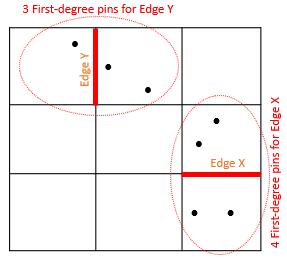
\includegraphics[width=.48\linewidth]{fdpin}  \label{fig:fdpin}}
    \subfloat[]{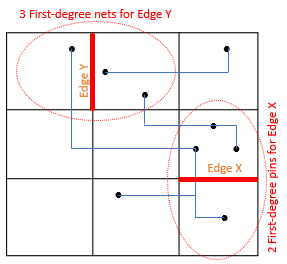
\includegraphics[width=.48\linewidth]{fdnet}  \label{fig:fdnet}}
    \caption{Examples of (a) first degree pins; (b) first degree nets;}
\end{figure}

\item \textbf{First-degree nets}. A tile can contain various pins which belong to different nets. Different pins in a tile can be a part of the same net or of different nets. Analogous to first degree pins, this attribute gives the number of nets that are closest to an edge. The first-degree nets of an edge are the nets that cross-over the space enclosed by either of the two tiles that the chosen edge is a part of \Cref{fig:fdnet}  gives an example of this attribute.

\item \textbf{Pin density}. This attribute makes use of First-degree pins to calculate the pin-density. It gives information regarding the number of pins per unit area. Pin density for a chosen edge is given by the number of first-degree pins divided by twice the tile area i.e., area of both tiles the edge is a part of. Pin density helps to give information of how congested the pins are within a tile which directly translates to a higher probability for the tile's corresponding edges to be used for routing. A higher pin density means that the edges of this tile can mostly be used to route pins within that tile. This deems the edges unroutable for wire connecting other tiles and thus a detour must be made. 

\item \textbf{RSMT-aware two-pin-pair usage}. This attribute assists in the evaluation of the most appropriate path for global routing based on a probabilistic model. The router initially creates multi-pin net Rectilinear Steiner Minimal Tree structures using the FLUTE \cite{FLUTE} and then fragments each structure into two-pin pairs. Having known the location of two pins, various paths are constructed from one to the other, as is shown in \Cref{fig:2pinusage}. Subsequently, the ‘total availability’ for each path is calculated. This total availability depends on the maximum capacity of each edge lying in the chosen path. Please note that the user has the freedom of choosing what paths to consider, such as L-shape, Z-shape and monotonic. More shapes considered provide enhanced accuracy, but comes with a runtime penalty.

\begin{figure}[tbh!]
    \centering
    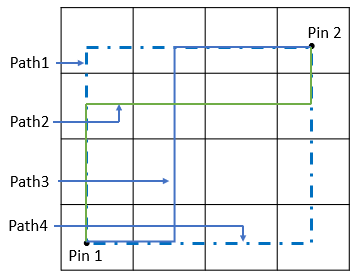
\includegraphics[width=1.5in]{2pinusage}
    \caption{Four possible paths for a two-pin pair.}
    \label{fig:2pinusage}
\end{figure}

If $n$ edges constitute path $i$, and let $M(e)$ be the maximum capacity for edge e, then the total availability $A(i)$ for path $i$ is $A(i)=\sum_{e=0}^{n}M(e)$. Following computation of the total availability of each of the potential paths, the probability of each path is calculated. This calculation is done by obtaining the sum of the total availability of all potential paths between the two pins as shown in \Cref{fig:2pinusage}.
If there are k paths, the probability of path $p(i)=\frac{A(i)}{\sum^{k}A}$

Each edge $j$ in path $i$ is assigned a probability $p(i)$ which reflects its likelihood for being used in global routing. Since an edge can belong to more than one potential path, the usage assigned to each edge is a sum of all the path probabilities of which this chosen edge is a part of. Thus, we acquire probabilistic information for each edge to be used in global routing. In an edge-based analyses, this attribute provides us valuable information for the routing probability of an edge from a standalone perspective.
\end{itemize}

\subsection{Routability-Driven Edge Shifting}
We use our routability information for the edge shifting technique in \cite{fastroute}. As is demonstrated in \Cref{fig:edgeshifting}, the congestion map heavily affects the structure of Steiner tree hence the actual routing. The quality of the congestion map as the guidance has to be taken care of.
\begin{figure}[htbp]
    \centerline{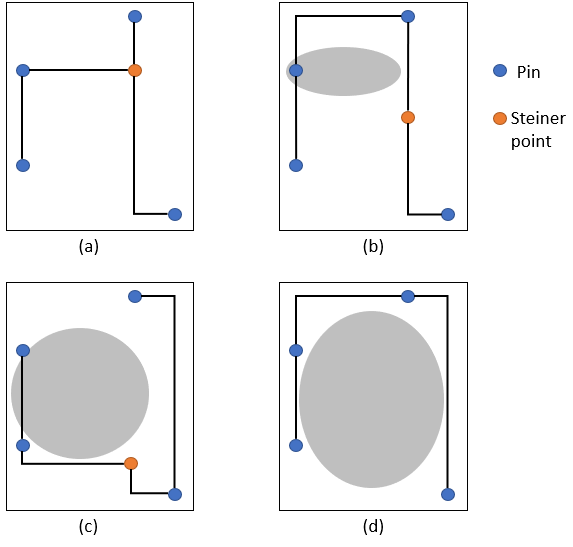
\includegraphics[height=2.1in, width=3in]{edgeshifting}}
    \caption{(a) The initial Steiner tree (b) Allowed moving area for Steiner point (c)(d) Modified tree structures based on different congestion map}
    \label{fig:edgeshifting}
\end{figure}


\subsection{Prediction Model Embedded Routability Optimization}
After the attributes are extracted, we use previously mentioned MARS \cite{MARS} to predict routability. The reasons of selecting MARS are as follows: 1) Interactions between independent parameters can be captured. 2) Non-linearity can be modeled. 3) Tunning is easy, and in most cases, not needed. 

The output congestion model from MARS is integrated into the global router. After necessary initialisation, FLUTE is performed to construct Steiner trees for each net. The congestion information is then input from the prediction of the congestion model, based on which the tree structure is further optimised and the initial routing executed. The guidance congestion map is removed before the rip-up and re-route stage because all paths are routed and the real congestion information is generated. Therefore the guidance is no longer needed as it will interfere the following process.

\begin{algorithm}
    \caption{Routability Model Guided Routing}
    \label{alg:route}
    \begin{algorithmic}[1]
        \Require Global Routing Instance.
        \State \texttt{Init()};
        \While{net $\gets$ nets.\texttt{read}()}
            \State \texttt{FLUTE}(net);
            \State congestion $\gets$ \texttt{inputGuide}(model);
            \State \texttt{edgeShifting}(net, congestion);
            \State \texttt{routing}(net, congestion);
            \State \texttt{removeGuide}(congestion);
            \While{FALSE == \texttt{metThreshold}()}
                \State \texttt{ripUpReroute}();
            \EndWhile
        \EndWhile
    \end{algorithmic}
\end{algorithm}

% \iffalse
% \begin{algorithm}
% \SetAlgoLined
% \KwResult{Global Routing Instance}
%  initialisation()\;
%  \While{net = nets.read()}{
%     FLUTE(net)\;
%     congestion = inputGuide(model)\;
%     edgeShifting(net, congestion)\;
%     routing(net, congestion)\;
%     removeGuide(congestion)\;
    
%     \While{!metThreshold()}{
%         ripUpReroute()\;
%         }
  
%  }
%  \caption{routability model guided routing}
% \end{algorithm}
% \fi
